\documentclass[tikz,border=5pt]{standalone}
\usepackage{amsmath}
\begin{document}

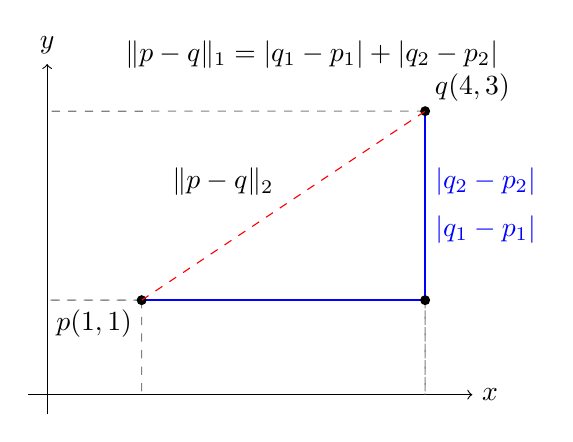
\begin{tikzpicture}[scale=1.2]
  % Axes
  \draw[->] (-0.2,0) -- (4.5,0) node[right] {$x$};
  \draw[->] (0,-0.2) -- (0,3.5) node[above] {$y$};

  % Points
  \coordinate (p) at (1,1);
  \coordinate (q) at (4,3);
  \coordinate (r) at (4,1); % intermediate corner for L1 path

  % Dashed grid lines
  \draw[dashed,gray] (p) -- (1,0);
  \draw[dashed,gray] (p) -- (0,1);
  \draw[dashed,gray] (q) -- (4,0);
  \draw[dashed,gray] (q) -- (0,3);
  \draw[dashed,gray] (r) -- (4,0);
  \draw[dashed,gray] (r) -- (0,1);

  % L1 path (axis-aligned)
  \draw[thick,blue] (p) -- (r) -- (q)
    node[midway,below right] {$|q_1-p_1|$}
    node[midway,above right] {$|q_2-p_2|$};

  % Points
  \fill (p) circle (1.5pt) node[below left] {$p(1,1)$};
  \fill (r) circle (1.5pt);
  \fill (q) circle (1.5pt) node[above right] {$q(4,3)$};

  % Optional diagonal (Euclidean) for comparison
  \draw[dashed,red] (p) -- (q)
    node[midway,above left,black] {$\|p-q\|_2$};

  % Equation label
  \node[align=center] at (2.8,3.6)
    {$\|p-q\|_1 = |q_1-p_1| + |q_2-p_2|$};

\end{tikzpicture}

\end{document}
